\appendix
\chapter{Notations}\label{App:A}
The following symbols are used in the thesis:
\begin{table}[h]
    \begin{tabular}{ll}
        $A, B, C$ & material parameters used for Paul-Mohr-Coulomb failure criterion \\
        $b$ & width of the prismatic specimen  \\
        $b_c$ & intercept of axisymmetric compression line in ($p-q$) plane \\
        $b_e$ & intercept of axisymmetric extension line in ($p-q$) plane \\
        $C_0$ & uniaxial compressive strength \\
        $c$ & cohesion \\
        $d$ & cylindrical specimen diameter \\
        $E$ & Young's modulus \\
        $err$ & distance between a data point and its fitted plane \\
        $h$ & specimen height \\
        $I_1$ & first invariant of stress state \\
        $J_2$ & second invariant of stress state \\
        $J_3$ & third invariant of stress state \\
        $k$ & slope of Paul-Mohr-Coulomb failure line in $\pi$-plane \\
        $K_p$ & slope of the Mohr-Coulomb failure line in $(\sigma_3-\sigma_1)$ plane \\
        $L$ & length of the prismatic specimen \\ 
        $M_c$ & slope of the Paul-Mohr-Coulomb compression line in $(\sigma_3-\sigma_1)$ plane \\
        $M_e$ & slope of the Paul-Mohr-Coulomb extension line in $(\sigma_3-\sigma_1)$ plane \\
        $MSE$ & mean square error \\
        $m$ & parameter for Hoek-Brown criterion \\
        $m_c$ & slope of the axisymmetric compression line in the $(p-q)$ plane\\
        $m_e$ & slope of the axisymmetric extension line in the $(p-q)$ plane\\
        $p$ & mean stress\\
        $p_c$ & mean stress of P1 and P2 intersection point in $(p-q)$ plane for compression \\
        $p_e$ & mean stress of P1 and P2 intersection point in $(p-q)$ plane for extension \\  
        $P1$ & plane 1 \\
        $P2$ & plane 2 \\
        $q$ & deviatoric stress \\
        $q_c$ & deviatoric stress for triaxial compression \\
        $q_e$ & deviatoric stress for triaxial extension \\
    \end{tabular}
\end{table}

\begin{table}
    \begin{tabular}{ll}
        $S_{ij}$ & deviator stress \\
        $\bar{S}$ & mean standard deviation misfit \\
        $s_i$ & standard deviation of the tests series $i$ \\
        $V_0$ & theoretical isotropic tensile strength \\
        $V_0^{(1)}$ & theoretical isotropic tensile strength for P1 \\
        $V_0^{(2)}$ & theoretical isotropic tensile strength for P2 \\
        $V_P$ & P-wave speed \\
        $x_1, x_2, x_3$ & component of the vector solution from least-square fitting\\
        $\alpha$ & $b_c/b_e$ \\
        $\delta_{ij}$ & Kronecker delta \\
        $\epsilon_{II}$ & intermediate principal strain \\
        $\epsilon_a$ & axial strain \\
        $\epsilon_l$ & lateral strain \\
        $\phi$ & friction angle \\
        $\phi^{(1)}$ & friction angle for P1 \\
        $\phi^{(2)}$ & friction angle for P2 \\
        $\phi_c$ & friction angle for axisymmetric compression \\
        $\phi_c^{(1)}$ & compression friction angle for P1 \\
        $\phi_c^{(2)}$ & compression friction angle for P2 \\
        $\phi_e$ & friction angle for axisymmetric extension \\
        $\phi_e^{(1)}$ & extension friction angle for P1 \\
        $\phi_e^{(2)}$ & extension friction angle for P2 \\
        $\nu$ & Poisson's ratio \\
        $\theta$ & Lode angle (angle from $\sigma_1^*$ in the $\pi$-plane) \\
        $\rho$ & dry density \\
        $\sigma$ & normal stress \\
        $\sigma_a$ & axial stress \\
        $\sigma_r$ & radial stress \\
        $\sigma_{ij}$ & stress component \\
        $\sigma_{1,2}$ & stress at the end of phase 1 of the constant mean stress true-triaxial experiment \\
        $\sigma_{I},\sigma_{II},\sigma_{III} $ & major, intermediate and minor principal stresses\\
        $\sigma_{1},\sigma_{2},\sigma_{3} $ & principal stresses with no regard to magnitude\\
        $\sigma_{1}^*,\sigma_{2}^*,\sigma_{3}^* $ & projection of the principal stress axes in $\pi$-plane \\
        $\sigma_{I,j}^{test}$ & major stress of data point $j$ \\
        $\sigma_{I,j}^{calc}$ & predicted major stress \\
        $\tau$ & shear stress \\
    \end{tabular}
\end{table}

\chapter{Failure criterion formulation in \texorpdfstring{$\pi$}{pi}-plane}\label{App:B}

The principal stresses, with no consideration for magnitude, are formulated in the $\pi$-plane as follow: 
\begin{align}
    \sigma_1 &= p + \frac{\sqrt{6}}{3}r\cos\left(\theta\right) \\
    \sigma_2 &= p - \frac{\sqrt{6}}{3}r\sin\left(\frac{\pi}{6}-\theta\right)\\
    \sigma_3 &= p - \frac{\sqrt{6}}{3}r\sin\left(\frac{\pi}{6}+\theta\right)
\end{align}

\section*{Mohr-Coulomb failure criterion}
The Mohr-Coulomb failure criterion is expressed in terms of the principal stresses $\sigma_I$ and $\sigma_{III}$:
\begin{equation}
    \sigma_I = K_p \sigma_{III} + C_0
\end{equation}
The formulation of the criterion in the $\pi$-plane is defined bellow for each possible ordering of stresses. On this plane, a point is at a distance $r$ from the origin of the hydrostatic axis and oriented at the Lodge angle $\theta$ from the  $\sigma_1^*$ axis.

Section (i) : $\sigma_I = \sigma_1$, $\sigma_{II} = \sigma_2$ and $\sigma_{III} = \sigma_3$

\begin{equation}
    r cos\theta = \frac{6}{2\sqrt{6}+\sqrt{6}K_p}\left[p(K_p-1)-\frac{\sqrt{2}}{2} K_p r sin\theta +C_0\right]
\end{equation}

Section (ii) : $\sigma_I = \sigma_2$, $\sigma_{II} = \sigma_1$ and $\sigma_{III} = \sigma_3$

\begin{equation}
    r cos\theta = \frac{6}{K_p \sqrt{6}-\sqrt{6}K_p}\left[p(K_p-1)-\frac{\sqrt{2}}{2} r sin\theta (1+K_p) +C_0\right]
\end{equation}

Section (iii) : $\sigma_I = \sigma_2$, $\sigma_{II} = \sigma_3$ and $\sigma_{III} = \sigma_1$

\begin{equation}
    r cos\theta = \frac{6}{2\sqrt{6}+\sqrt{6}K_p}\left[p(K_p-1)+\frac{\sqrt{2}}{2} r sin\theta -C_0\right]
\end{equation}

Section (iv) : $\sigma_I = \sigma_3$, $\sigma_{II} = \sigma_2$ and $\sigma_{III} = \sigma_1$

\begin{equation}
    r cos\theta = \frac{6}{2\sqrt{6}+\sqrt{6}K_p}\left[p(K_p-1)-\frac{\sqrt{2}}{2} r sin\theta -C_0\right]
\end{equation}

Section (v) : $\sigma_I = \sigma_3$, $\sigma_{II} = \sigma_1$ and $\sigma_{III} = \sigma_2$

\begin{equation}
    r cos\theta = \frac{6}{K_p \sqrt{6}-\sqrt{6}K_p}\left[p(K_p-1)+\frac{\sqrt{2}}{2} r sin\theta (1+K_p) +C_0\right]
\end{equation}

Section (vi) : $\sigma_I = \sigma_1$, $\sigma_{II} = \sigma_3$ and $\sigma_{III} = \sigma_2$

\begin{equation}
    r cos\theta = \frac{6}{2\sqrt{6}+\sqrt{6}K_p}\left[p(K_p-1)+K_p \frac{\sqrt{2}}{2} r sin\theta +C_0\right]
\end{equation}

\section*{Hoek-Brown failure criterion}
The Hoek-Brown failure criterion is expressed in terms of the principal stresses $\sigma_I$ and $\sigma_{III}$:
\begin{equation}
    \sigma_I = \sigma_{III} + C_0 \sqrt{\frac{m}{C_0} \sigma_{III}+1}
\end{equation}
The formulation of the criterion in the $\pi$-plane is defined bellow for each possible ordering of stresses. On this plane, a point is at a distance $r$ from the origin of the hydrostatic axis and oriented at the Lodge angle $\theta$ from the  $\sigma_1^*$ axis.

Section (i) : $\sigma_I = \sigma_1$, $\sigma_{II} = \sigma_2$ and $\sigma_{III} = \sigma_3$

\begin{equation}
    r cos\theta = \frac{2}{\sqrt{6}}\left[-\frac{\sqrt{2}}{2} r sin\theta + C_0 \sqrt{\frac{m}{C_0} \left(p-\frac{\sqrt{6}}{6} r cos\theta - \frac{\sqrt{2}}{2} r sin\theta \right)+1}\right]
\end{equation}

Section (ii) : $\sigma_I = \sigma_2$, $\sigma_{II} = \sigma_1$ and $\sigma_{III} = \sigma_3$

\begin{equation}
    r cos\theta = \sqrt{6}\left[p-\frac{\sqrt{2}}{2} r sin\theta + \frac{C_0^2-2 r^2 sin^2\theta}{C_0 m}\right]
\end{equation}

Section (iii) : $\sigma_I = \sigma_2$, $\sigma_{II} = \sigma_3$ and $\sigma_{III} = \sigma_1$

\begin{equation}
    r cos\theta = \frac{2}{\sqrt{6}}\left[\frac{\sqrt{2}}{2} r sin\theta - C_0 \sqrt{\frac{m}{C_0} \left(p+\frac{\sqrt{6}}{3} r cos\theta \right)+1}\right]
\end{equation}

Section (iv) : $\sigma_I = \sigma_3$, $\sigma_{II} = \sigma_2$ and $\sigma_{III} = \sigma_1$

\begin{equation}
    r cos\theta = \frac{2}{\sqrt{6}}\left[-\frac{\sqrt{2}}{2} r sin\theta - C_0 \sqrt{\frac{m}{C_0} \left(p+\frac{\sqrt{6}}{3} r cos\theta \right)+1}\right]
\end{equation}

Section (v) : $\sigma_I = \sigma_3$, $\sigma_{II} = \sigma_1$ and $\sigma_{III} = \sigma_2$

\begin{equation}
    r cos\theta = \sqrt{6}\left[p+\frac{\sqrt{2}}{2} r sin\theta + \frac{C_0^2-2 r^2 sin^2\theta}{C_0 m}\right]
\end{equation}

Section (vi) : $\sigma_I = \sigma_1$, $\sigma_{II} = \sigma_3$ and $\sigma_{III} = \sigma_2$

\begin{equation}
    r cos\theta = \frac{2}{\sqrt{6}}\left[\frac{\sqrt{2}}{2} r sin\theta + C_0 \sqrt{\frac{m}{C_0} \left(p-\frac{\sqrt{6}}{6} r cos\theta + \frac{\sqrt{2}}{2} r sin\theta \right)+1}\right]
\end{equation}

\section*{Paul-Mohr-Coulomb failure criterion}
The Paul-Mohr-Coulomb failure criterion is expressed in terms of the principal stresses $\sigma_I$, $\sigma_{II}$ and $\sigma_{III}$:
\begin{equation}
    A \sigma_I + B \sigma_{II} + C \sigma_{III} = 1
\end{equation}
The formulation of the criterion in the $\pi$-plane is defined bellow for each possible ordering of stresses. On this plane, a point is at a distance $r$ from the origin of the hydrostatic axis and oriented at the Lodge angle $\theta$ from the  $\sigma_1^*$ axis.

Section (i) : $\sigma_I = \sigma_1$, $\sigma_{II} = \sigma_2$ and $\sigma_{III} = \sigma_3$

\begin{equation}
    r cos\theta = \frac{6}{\sqrt{6}(2A-B-C)} \left[ 1-p(A+B+C)- \frac{\sqrt{2}}{2} r sin \theta (B+C) \right]
\end{equation}

Section (ii) : $\sigma_I = \sigma_2$, $\sigma_{II} = \sigma_1$ and $\sigma_{III} = \sigma_3$

\begin{equation}
    r cos\theta = \frac{6}{\sqrt{6}(2B-A-C)} \left[ 1-p(A+B+C)+ \frac{\sqrt{2}}{2} r sin \theta (C-A) \right]
\end{equation}

Section (iii) : $\sigma_I = \sigma_2$, $\sigma_{II} = \sigma_3$ and $\sigma_{III} = \sigma_1$

\begin{equation}
    r cos\theta = \frac{6}{\sqrt{6}(2C-A-B)} \left[ 1-p(A+B+C)+ \frac{\sqrt{2}}{2} r sin \theta (B-A) \right]
\end{equation}

Section (iv) : $\sigma_I = \sigma_3$, $\sigma_{II} = \sigma_2$ and $\sigma_{III} = \sigma_1$

\begin{equation}
    r cos\theta = \frac{6}{\sqrt{6}(2C-B-A)} \left[ 1-p(A+B+C)+ \frac{\sqrt{2}}{2} r sin \theta (A-B) \right]
\end{equation}

Section (v) : $\sigma_I = \sigma_3$, $\sigma_{II} = \sigma_1$ and $\sigma_{III} = \sigma_2$

\begin{equation}
    r cos\theta = \frac{6}{\sqrt{6}(2B-A-C)} \left[ 1-p(A+B+C)+ \frac{\sqrt{2}}{2} r sin \theta (A-C) \right]
\end{equation}

Section (vi) : $\sigma_I = \sigma_1$, $\sigma_{II} = \sigma_3$ and $\sigma_{III} = \sigma_2$

\begin{equation}
    r cos\theta = \frac{6}{\sqrt{6}(2A-B-C)} \left[ 1-p(A+B+C)+ \frac{\sqrt{2}}{2} r sin \theta (B-C) \right]
\end{equation}


\chapter{Fitting program}\label{App:C}

The resources of the program developed for failure criteria fitting are available at the following address: https://github.com/hfuselier/PDM/tree/master/python.

Its objective is to provide a fitting solution and representations of the failure surface in a three-dimensional space and in the $\pi$-plane for the Paul-Mohr-Coulomb failure criterion. The development of the program was considered to enable the fitting of the three-parameter, six-parameter and simplified Paul-Mohr-Coulomb criterion. The "\_README.pdf" file explains how to use the program for the evaluation  of the Paul-Mohr-Coulomb failure criterion and its comparison with the Mohr-Coulomb and Hoek-Brown failure criteria. 

The files gather in the "python" folder are organized as presented in Table \ref{tbC:files}.
\begin{table}[!b]
    \centering
    \caption{Organization of the program}
    \begin{tabular}{ll}
        \hline
        Application & Associated files\\
        \hline
        \hline
        Paul-Mohr-Coulomb with three parameters & $pmc.py$,\\
         & $brute\_force.py$, \\
         & $error\_computation.py$,\\
         & $Plot\_one\_plane.ipynb$\\
         \\
        Paul-Mohr-Coulomb with six parameters & $pmc.py$, \\
         & $brute\_force.py$, \\
         & $error\_computation.py$,\\
         & $Plot\_3D\_6-12-6.ipynb$\\
        \\
        Simplified Paul-Mohr-Coulomb & $pmc\_4p.py$,\\
        & $brute\_force\_4p.py$, \\
        & $error\_computation\_4p.py$,\\
        & $Plot\_3D\_6-12-6.ipynb$\\
       \\
    \end{tabular}
    \label{tbC:files}
\end{table}
\begin{table}
    \centering
    \begin{tabular}{ll}
        \hline
        Application & Associated files\\
        \hline
        \hline
        Mohr-Coulomb fitting with all data & $mc.py$, \\
         & $error\_computation.py$,\\
         & $Plot\_one\_plane.ipynb$\\
        \\
        Hoek-Brown fitting with all data & $hb.py$, \\
         & $error\_computation.py$,\\
         & $Plot\_one\_plane.ipynb$\\
        \\
        Mohr-Coulomb fitting with six data & $mc.py$, \\
         & $error\_computation\_4p.py$,\\
         & $Plot\_one\_plane.ipynb$\\
        \\
        Hoek-Brown fitting with six data & $hb.py$, \\
         & $error\_computation\_4p.py$,\\
         & $Plot\_one\_plane.ipynb$
    \end{tabular}
\end{table}


\chapter{Paul-Mohr-Coulomb failure surface}\label{App:D}

\begin{figure}[!ht]
    \centering
    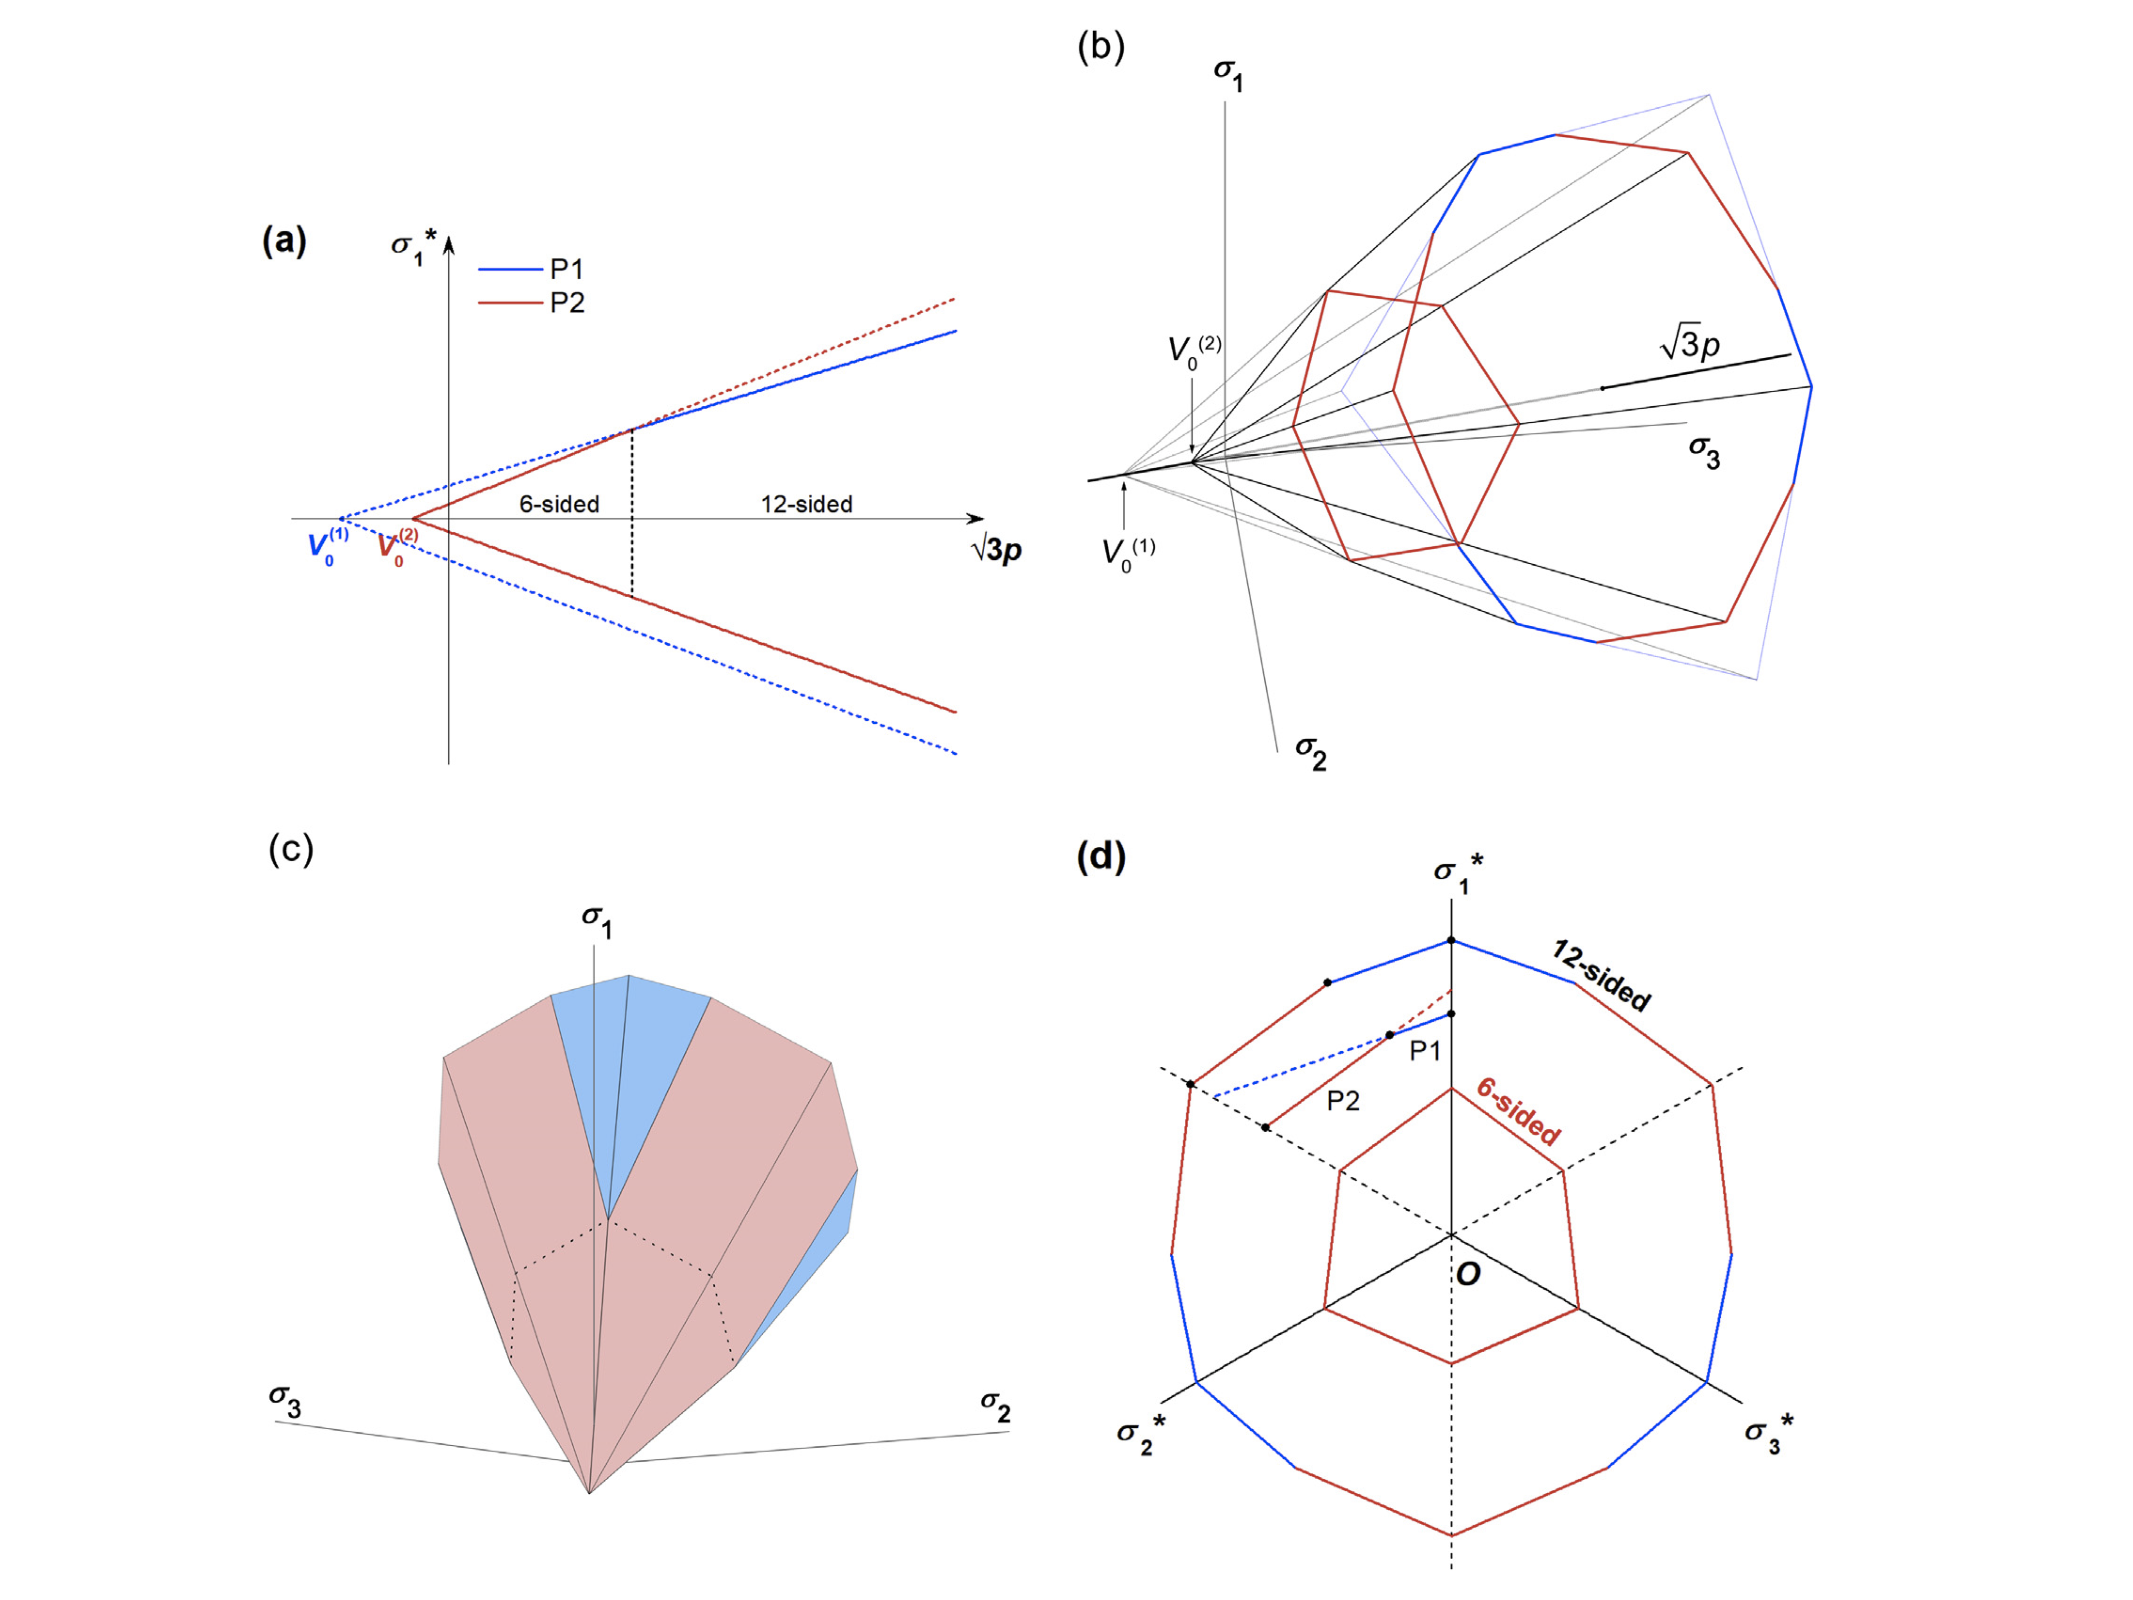
\includegraphics[width=0.94\columnwidth]{6pmc_typeiii}
    \captionsetup{justification=centering}
    \caption{Six-parameter Paul-Mohr-Coulomb featuring the evolution of the 6 sided to 12 sided pyramidal failure surface in the (a) $\sqrt{3}p - \sigma_1^*$ plane; (b) principal stress space, transparent view; (c) principal stress space, opaque view; (d) $\pi$-plane \cite{Labuz2018}}
    \label{fig5:6pmc_typeiii}
\end{figure}

\begin{figure}[!ht]
    \centering
    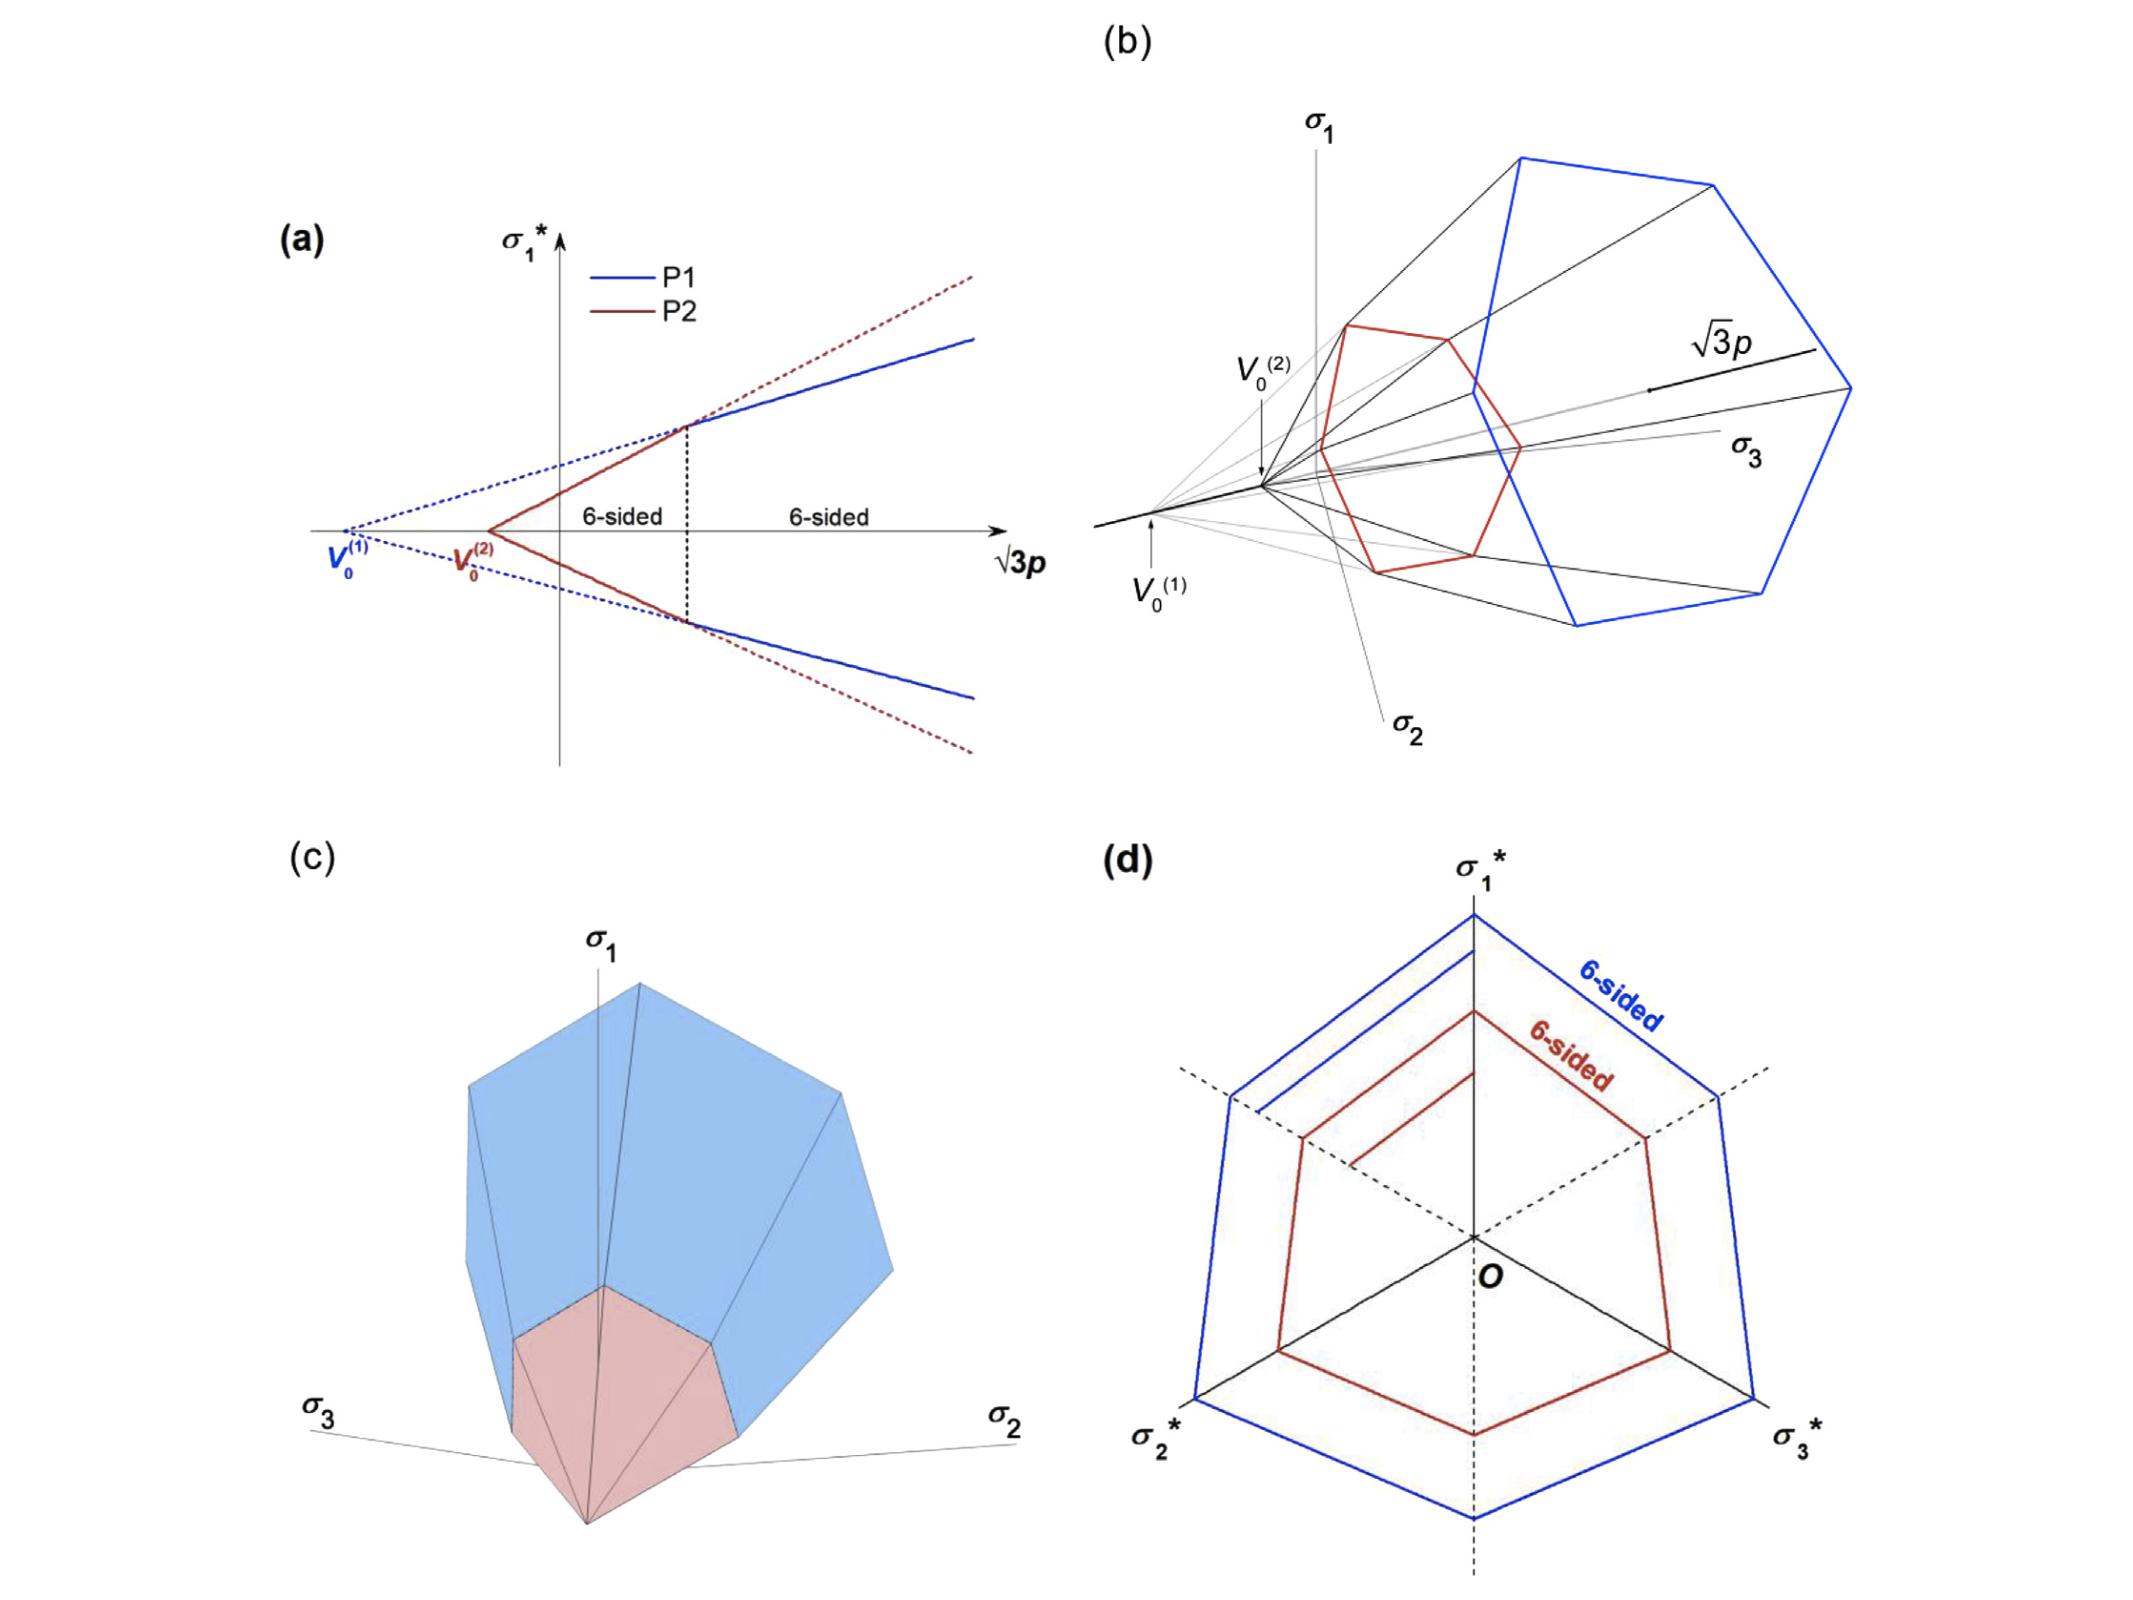
\includegraphics[width=\columnwidth]{6pmc_typeiv}
    \captionsetup{justification=centering}
    \caption{Six-parameter Paul-Mohr-Coulomb featuring the evolution of the 6 sided to 6 sided pyramidal failure surface in the (a) $\sqrt{3}p - \sigma_1^*$ plane; (b) principal stress space, transparent view; (c) principal stress space, opaque view; (d) $\pi$-plane \cite{Labuz2018}}
    \label{fig5:6pmc_typeiv}
\end{figure}

\chapter{Paul-Mohr-Coulomb failure criteria for rocks from literature}\label{App:E}

The Paul-Mohr-Coulomb failure criterion was evaluated for rocks with published data (from Labuz et al. (2018) \cite{Labuz2018}) that provide a 6-12-6 failure surface. The obtained results are presented in Table \ref{AppE:litt_rock}.





\begin{table}[!ht]
    \centering 
    \captionsetup{justification=centering}
    \caption{Values of the six PMC parameters for selected rock with a 6-12-6 sided failure surface}
    \begin{tabular}{lcccccc}
        \hline
        Rock & $V_0^{(1)}$ [\si{\mega\pascal}] & $\phi_c^{(1)}$ [\si{\degree}] & $\phi_e^{(1)}$ [\si{\degree}] & $V_0^{(2)}$ [\si{\mega\pascal}] & $\phi_c^{(2)}$ [\si{\degree}] & $\phi_c^{(2)}$ [\si{\degree}]\\
        \hline
        \hline
        Darley Dale sandstone & 76.3 & 30.9 &  32.2 & 18.3 & 44.9 & 48.4 \\
        Berea sandstone & 84.1 & 28.3 &  25.9 & 13.2 & 47.7 & 53.0 \\
        Indiana limestone & 31.0 & 27.2 &  28.1 & 9.68 & 43.9 & 44.3 \\
        Taiwan siltstone & 61.3 & 28.8 &  28.9 & 10.5 & 48.4 & 39.8 \\
        Coconino sandstone & 50.7 & 36.8 &  36.8 & 7.81 & 53.3 & 55.1 \\
        Bentheim sandstone & 27.3 & 33.5 &  34.5 & 9.44 & 37.7 & 43.1 \\
    \end{tabular}
    \label{AppE:litt_rock}
\end{table}


